\documentclass{article}

\usepackage{fancyhdr}
\usepackage{extramarks}
\usepackage{amsmath}
\usepackage{amsthm}
\usepackage{amsfonts}
\usepackage{tikz}
\usepackage[plain]{algorithm}
\usepackage{algpseudocode}
\usepackage{enumerate}
\usepackage{tikz}
\usepackage{listings}
\usepackage{hyperref}
\usepackage{subfigure}
\usepackage[graphicx]{realboxes}
\usepackage{xcolor}


% 代码块高级设置
\lstset{
% basicstyle=\footnotesize,                 % 设置整体的字体大小
showstringspaces=false,                     % 不显示字符串中的空格
frame=single,                               % 设置代码块边框
numbers=left,                               % 在左侧显示行号
% numberstyle=\footnotesize\color{gray},    % 设置行号格式
numberstyle=\color{darkgray},               % 设置行号格式
backgroundcolor=\color{white},              % 设置背景颜色
keywordstyle=\color{blue},                  % 设置关键字颜色
commentstyle=\it\color[RGB]{0,100,0},       % 设置代码注释的格式
stringstyle=\sl\color{red},                 % 设置字符串格式
}

\hypersetup{hidelinks,
	colorlinks=true,
	allcolors=black,
	pdfstartview=Fit,
	breaklinks=true}


%new command
\newcommand{\genstirlingI}[3]{%
  \genfrac{[}{]}{0pt}{#1}{#2}{#3}%
}
\newcommand{\genstirlingII}[3]{%
  \genfrac{\{}{\}}{0pt}{#1}{#2}{#3}%
}
\newcommand{\stirlingI}[2]{\genstirlingI{}{#1}{#2}}
\newcommand{\dstirlingI}[2]{\genstirlingI{0}{#1}{#2}}
\newcommand{\tstirlingI}[2]{\genstirlingI{1}{#1}{#2}}
\newcommand{\stirlingII}[2]{\genstirlingII{}{#1}{#2}}
\newcommand{\dstirlingII}[2]{\genstirlingII{0}{#1}{#2}}
\newcommand{\tstirlingII}[2]{\genstirlingII{1}{#1}{#2}}

\usetikzlibrary{automata,positioning}

%
% Basic Document Settings
%  

\topmargin=-0.45in
\evensidemargin=0in
\oddsidemargin=0in
\textwidth=6.5in
\textheight=9.0in
\headsep=0.25in

\linespread{1.1}

\pagestyle{fancy}
\lhead{\hmwkAuthorName}
\chead{\hmwkClass : \hmwkTitle}
\rhead{\firstxmark}
\lfoot{\lastxmark}
\cfoot{\thepage}

\renewcommand\headrulewidth{0.4pt}
\renewcommand\footrulewidth{0.4pt}

\setlength\parindent{0pt}

%
% Create Problem Sections
%

\newcommand{\enterProblemHeader}[1]{
    \nobreak\extramarks{}{Problem \arabic{#1} continued on next page\ldots}\nobreak{}
    \nobreak\extramarks{Problem \arabic{#1} (continued)}{Problem \arabic{#1} continued on next page\ldots}\nobreak{}
}

\newcommand{\exitProblemHeader}[1]{
    \nobreak\extramarks{Problem \arabic{#1} (continued)}{Problem \arabic{#1} continued on next page\ldots}\nobreak{}
    \stepcounter{#1}
    \nobreak\extramarks{Problem \arabic{#1}}{}\nobreak{}
}

\newcommand*\circled[1]{\tikz[baseline=(char.base)]{
		\node[shape=circle,draw,inner sep=2pt] (char) {#1};}}
\newcommand{\ts}{\textsuperscript}

\setcounter{secnumdepth}{0}
\newcounter{partCounter}
\newcounter{homeworkProblemCounter}
\setcounter{homeworkProblemCounter}{1}
\nobreak\extramarks{yuzhh1@shanghaitech.edu.cn}{}\nobreak{}

%
% Homework Problem Environment
%
% This environment takes an optional argument. When given, it will adjust the
% problem counter. This is useful for when the problems given for your
% assignment aren't sequential. See the last 3 problems of this template for an
% example.
%

\newenvironment{homeworkProblem}[1][-1]{
    \ifnum#1>0
        \setcounter{homeworkProblemCounter}{#1}
    \fi
    \section{Page \arabic{homeworkProblemCounter}}
    \setcounter{partCounter}{1}
    \enterProblemHeader{homeworkProblemCounter}
}{
    \exitProblemHeader{homeworkProblemCounter}
}

%
% Homework Details
%   - Title
%   - Due date
%   - Class
%   - Instructor
%   - Class number
%   - Name
%   - Student ID

\newcommand{\hmwkTitle}{Lab 0 Report}
\newcommand{\hmwkDueDate}{September 23rd}
\newcommand{\hmwkClass}{Advanced Computer Architecture}
\newcommand{\hmwkClassInstructor}{Professor Chundong Wang}

% 正式选课名单确定之后,根据通知填写所在班级编号

\newcommand{\hmwkAuthorName}{Zhenghong Yu}
\newcommand{\hmwkAuthorMail}{yuzhh1@shanghaitech.edu.cn}
\newcommand{\hmwkAuthorID}{2020533156}


%
% Title Page
%

\title{
    \vspace{2in}
    \textmd{\textbf{\hmwkClass:\\  \hmwkTitle}}\\
    \normalsize\vspace{0.1in}\small{Due\ on\ \hmwkDueDate\ at 11:59am}\\
   \vspace{2in}
}

\author{
	Name: \textbf{\hmwkAuthorName} \\
    Mailbox: \textbf{\hmwkAuthorMail} \\
	Student ID: \hmwkAuthorID}
\date{}

\renewcommand{\part}[1]{\textbf{\large Part \Alph{partCounter}}\stepcounter{partCounter}\\}

%
% Various Helper Commands
%

% Useful for algorithms
\newcommand{\alg}[1]{\textsc{\bfseries \footnotesize #1}}
% For derivatives
\newcommand{\deriv}[1]{\frac{\mathrm{d}}{\mathrm{d}x} (#1)}
% For partial derivatives
\newcommand{\pderiv}[2]{\frac{\partial}{\partial #1} (#2)}
% Integral dx
\newcommand{\dx}{\mathrm{d}x}
% Alias for the Solution section header
\newcommand{\solution}{\textbf{\large Solution}}
% Probability commands: Expectation, Variance, Covariance, Bias
\newcommand{\E}{\mathrm{E}}
\newcommand{\Var}{\mathrm{Var}}
\newcommand{\Cov}{\mathrm{Cov}}
\newcommand{\Bias}{\mathrm{Bias}}

\begin{document}

\maketitle
\pagebreak
\tableofcontents

\pagebreak



\section{Realize LR and SC in simulator}
\subsection{Requirement of LR and SC}
\subsubsection{Premise}
The content below based on the \textbf{"A" Standard Extention for Atomic Instructions, Version 2.1} which is the newest version on the wiki.riscv.org.\\
\subsubsection{Details}
$\cdot$     LR and SC are both 32-bits instructions with opcode $0x2F$, funct5 (which means the last 5 bits number of the instruction) is $0x3$ for $8$ bytes data and $0x2$ for $4$ bytes data. Additionally, we dont need to consider aligned data, number limitation between LR and SC.\\\\
$\cdot$     LR loads a data from the address in $rs1$, places the \textbf{sign-extended} value in $rd$, and registers \textbf{a reservation set}—a set of bytes that subsumes the bytes in the addressed word. \\\\
$\cdot$     SC conditionally writes a data in $rs2$ to the address in $rs1$: the SC succeeds only if the reservation is still \textbf{valid} and the reservation set contains the
bytes being written. If the SC succeeds, the instruction writes the data in $rs2$ to memory, and it writes \textbf{zero} to $rd$. If the SC fails, the instruction does \textbf{not} write to memory, and it writes a \textbf{nonzero} value to $rd$. Regardless of success or failure, executing an SC instruction invalidates \textbf{any} reservation held by this hart. \\\\
$\cdot$     An SC can only \textbf{pair with} the \textbf{most recent} LR in program order. An SC may succeed only if \textbf{no store} from another hart to the reservation set can be observed to have occurred between the LR and the SC, and if there is \textbf{no other} SC between the LR and itself in program order. An SC may succeed only if no write from a device other than a hart to the bytes accessed by the LR instruction can be observed to have occurred between the LR and SC. Note this LR might have had a different effective address and data size, but reserved the SC's address as part of the reservation set.\\\\
$\cdot$     The SC must \textbf{fail} if the address is not within the reservation set of the \textbf{most recent} LR in program order. The SC must \textbf{fail} if a store to the reservation set from another hart can be observed to occur between the LR and SC. The SC must \textbf{fail} if a write from some other device to the bytes accessed by the LR can be observed to occur between the LR and SC. An SC must \textbf{fail} if there is another SC (to any address) between the LR and the SC in program order.\\\\

$\cdot$     The failure code with value \textbf{1} is reserved to encode an unspecified failure. Other failure codes are reserved at this time, and portable software should only assume the failure code will be non-zero. \\\\
$\cdot$     To other access memory operations (\textbf{Load} or \textbf{Store}), we only concern about store instruction which access to these addresses that have been already reserved, remove these addresses from the reservation set.
\subsection{Idea}
$\cdot$ I use \textbf{registry\_addr} to record the first address, \textbf{registry\_whe} to record whether the reservation set is still valid, \textbf{registry\_num} to record the length of the reservation set. These is declared in the $Simulator.h$.\\\\
$\cdot$ I almost use the datapath of \textbf{Load} instruction and \textbf{Store} instruction, as they have the same hazard which can handle samely.\\\\
$\cdot$ Specially, despite the instruction fetch and datapath set, I handle the most important part (reserve and check) in the $class memoryAccess$, which I think it might be more easier to be realize on hardware.\\\\ 
\subsection{Implementation}
New variable or modification statement in $Simulator.h$
\begin{lstlisting}[language=c++]
    ......
    namespace RISCV
    {
        ......
        enum Inst
        {
            ......
            LRW = 54,   /* add encode lr.w instruction as 54 */
            LRD = 55,   /* add encode lr.d instruction as 55 */
            SCW = 56,   /* add encode sc.w instruction as 56 */
            SCD = 57,   /* add encode sc.d instruction as 57 */
            ......
        };
        ......
        /* add LR SC instruction with opcode 0X2F */
        const int OP_CAS = 0x2F;
        ......
        inline bool isReadMem(Inst inst)
        {
            /* As LR and SC both need memory access and write back to 
               reg, so we need to handle with harzard in pipline */
            if (...... || inst == LRW || inst == LRD
                || inst == SCW || inst == SCD)
            {
                return true;
            }
            return false;
        } 
    }

    class Simulator
    {
    public:
        ......
    private:
        ......
        struct EReg
        {
            ......
            bool _cas;
        } eReg, eRegNew;
        ......
        uint32_t registry_addr; /* Registry hold the first address */ 
        uint32_t registry_num;  /* Registry hold the number */
        bool registry_whe;      /* Registry hold the valid bit */
    }


\end{lstlisting}
New variable or modification statement in $Simulator.cpp$
\begin{lstlisting}[language=c++]
    ......
    namespace RISCV
    {
        ......
        const char *INSTNAME[]{ /* add instruction name */
            ......,"lrw","lrd","scw","scd"};
    }
    ......
    void Simulator::decode()
    {
        ......
        if (this->fReg.len == 4) // 32 bit instruction
        {
            ......
            switch (opcode)
            {
                ......
                case OP_CAS: /* add OP_CAS handler */
                {
                    /* read data in reg[rs1] which store the address */
                    op1 = this->reg[rs1]; 
                    /* read data in reg[rs2] which is no mean in LR, 
                        store the old_value in SC */
                    op2 = this->reg[rs2]; 
                    reg1 = rs1;
                    reg2 = rs2;
                    dest = rd;  /* The reg which should be write back */

                    /* Get the funct5 */
                    uint32_t  temp = (inst >> 27) & 0x1F;
                    switch (temp)
                    {
                    case 0x2:   /* LR instruction */
                        if (funct3 == 3)    /* LR.D instruction */
                        {
                            instname = "lrd";
                            insttype = LRD;
                        }
                        else if (funct3 == 2)   /* LR.W instruction */
                        {
                            instname = "lrw";
                            instyype = LRW;
                        }
                        else
                        {
                            this->panic("Unknown 32bit funct3 
                                0x%x\n", funct3);
                        }
                        break;
                    case 0x3:   /* SC instruction */
                        if (funct3 == 3)    /* SC.D instruction */
                        {
                            instname = "scd";
                            insttype = SCD;
                        }
                        else if (funct3 == 2)   /* SC.W instruction */
                        {
                            instname = "scw";
                            instyype = SCW;
                        }
                        else
                        {
                            this->panic("Unknown 32bit funct3
                                0x%x\n", funct3);
                        }
                        break;
                    default:
                        this->panic("Unknown 32bit funct5
                            0x%x\n", temp);
                    }
                }
                ......
            }
        }
        ......
    }

    void Simulator::excecute()
    {
        ......
        bool _cas = false;  /* To identify whether it is a LR or SC */

        switch (inst)
        {
            ......
            case LRW:   /* Datapath of LR.W instruction */
                readMem = true;
                writeReg = true;
                memLen = 4;
                out = op1;
                readSignExt = true;
                _cas = true;
                break;
            case LRD:   /* Datapath of LR.D instruction */
                readMem = true;
                writeReg = true;
                memLen = 8;
                out = op1;
                readSignExt = true;
                _cas = true;
                break;
            case SCW:   /* Datapath of SC.W instruction */
                writeReg = true;
                writeMem = true;
                memLen = 4;
                out = op1;
                _cas = true;
                op2 = op2 & 0xFFFFFFFF;
                break;
            case SCD:   /* Datapath of SC.D instruction */
                writeReg = true;
                writeMem = true;
                memLen = 8;
                out = op1;
                op2 = op2 & 0xFFFFFFFF;
                _cas = true;
                break;
            ......
        }
        ......
        /* Pass the information to the next stage */
        this->eRegNew._cas = _cas;  
    }

    void Simulator::memoryAccess()
    {
        ......
        bool _cas = this->eReg._cas;
        ......
        if (writeMem)
        {
            switch (memLen)
            {
            case 1:
                good = this->memory->setByte(out, op2, &cycles);
                if ((out >= this->registry_addr) && (out <=
                    (this->registry_addr + this->registry_num))) 
                {   /* If there is any byte write to the reservation set */
                    this->registry_whe = false;
                }
                break;
            case 2:
                good = this->memory->setShort(out, op2, &cycles);
                for (uint32_t i = 0; i < 2; i++) 
                {
                    if (((out + i) >= this->registry_addr) && ((out + i) 
                        <= (this->registry_addr + this->registry_num)))
                    {   /* Any byte write to the reservation set */
                        this->registry_whe = false;
                    }
                }
                break;
            case 4:
                if (_cas)
                {   /* If this is SC instruction */
                    if (this->registry_whe && (this->registry_addr 
                        == out) && (this->registry_num == 4))
                    {   /* Reservation set is valid 
                            the first address same
                            the access length same */
                        good = this->memory->setInt(out, op2, &cycles);
                        out = 0;
                    }
                    else
                    {   /* If failed return code 1 */
                        out = 1;
                    }
                    /* SC eliminate all reservation */
                    this->registry_whe = false;
                }
                else
                {   /* If not, do basic store operation */
                    for (uint32_t i = 0; i < 4; i++) 
                    {   /* For all bytes */
                        if (((out + i) >= this->registry_addr) && 
                            ((out + i) <= (this->registry_addr +
                            this->registry_num)))
                        {   /* Any access to the bytes */
                            this->registry_whe = false;
                        }
                    }
                    good = this->memory->setInt(out, op2, &cycles);
                }
                break;
            case 8:
                if (_cas)
                {
                    if (this->registry_whe && (this->registry_addr 
                        == out) && (this->registry_num == 8))
                    {   /* Reservation set is valid
                            the first address same
                            the access length same */
                        good = this->memory->setLong(out, op2, &cycles);
                        out = 0;
                    }
                    else
                    {
                        out = 1;
                    }
                    tthis->registry_whe = false;
                }
                else
                {
                    for (uint32_t i = 0; i < 8; i++) 
                    {
                        if (((out + i) >= this->registry_addr) 
                            && ((out + i) <= (this->registry_addr 
                            + this->registry_num)))
                        {
                            this->registry_whe = false;
                        }
                    }
                    good = this->memory->setLong(out, op2, &cycles);
                }
            }
        }
        ......
        if (readMem)
        {   /* Handle with LR instruction */
            switch (memLen)
            {
                ......
            case 4: 
                if(readSignExt)
                {
                    if(_cas)
                    {   /* LR.W instruction */
                        this->registry_whe = true;  /* Valid */
                        this->registry_addr = out;  /* Store */
                        this->registry_num = 4; /* Length */
                    }
                    out = (int64_t)this->memory->getInt(out, &cycles);
                }
                ......
            case 8:
                if(readSignExt)
                {
                    if(_cas)
                    {   /* LR.W instruction */
                        this->registry_whe = true;
                        this->registry_addr = out;
                        this->registry_num = 8;
                    }
                    out = (int64_t)this->memory->getInt(out, &cycles);
                }
                ......

            }

        }
    }


\end{lstlisting}

\section{Realize CAS in lab0.c}
\subsection{Requirement of CAS}
\subsubsection{Details}
$\cdot$ Input of function is three variables: address which we want to store, old value that we think it should be, new value that we want to store in the address.\\\\
$\cdot$ We first load the value from the address, compare to the old value, if they are same (means until now, this address is not modified), store the new value into it and return code 1(true), if they are not same (means it has already been modified), stop store and return code 0(false).\\\\
$\cdot$ To make sure the CAS operation would not been interrupted, we must use \textbf{LR} instruction to load and \textbf{SC} instruction to store, in order to make sure the content of the perticular address would not be modified while doing CAS operation. If \textbf{SC} failed, just try again until success.
\subsection{Idea}
$\cdot$ I use inline assembler to make sure that it will use $LR$ and $SC$ instruction. Also use keyword \textbf{\_\_volatile\_\_} to make sure that the assembler will not optimize my code.\\\\
\subsection{Implementation}
\begin{lstlisting}[language=c++]
int CAS(long *dest, long new_value, long old_value)
{
    int ret = 0;

    // TODO: write your code here
    __asm__ __volatile__(
        "retry: lr.w  %0, %[output2]\n" /* Load value of addr */
        "       bne   %0, %[input1], fail\n" /* Compare and check */
        "       sc.w  %0, %[input2], %[output2]\n" /* Store new value */
        "       bnez  %0, retry\n"  /* Whether atom operation succcess */
        "       li    %[output1], 1\n"  /* Return code 1 */
        "       j     success\n"    /* Go on following */
        "fail:  li    %[output1], 0\n"  /* Return code 0 */
        "success: \n"
        : [output1] "=&r"(ret), [output2] "+A"(*dest)
        : [input1] "rJ"(old_value), [input2] "rJ"(new_value)
        : "memory");

    return ret;
}
\end{lstlisting}
\pagebreak
\section{Result}
I compile $lab0.c$ and run it, the following result is correct(some debug output, just ignore it), the first circulation should be failed, the second circulation should be success and store new value into the address.
\begin{figure}[!h]
\centering 
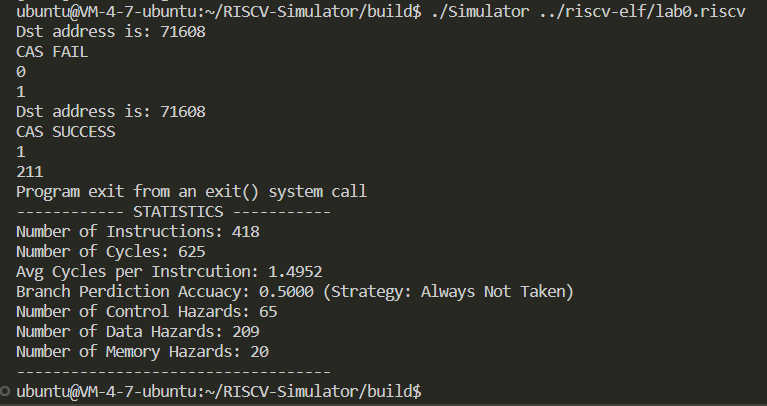
\includegraphics[height=8.5cm,width=14cm]{result.png}
\end{figure}

\section{Verification}
I check the whole process and write some simple other test to my implementation, I believe it is right.

\end{document}
